\documentclass[10pt,landscape,letterpaper,twoside]{article}
\usepackage[utf8]{inputenc}
\usepackage[T1]{fontenc}
\usepackage{lmodern}
%\usepackage[LY1,T1]{fontenc}
%\usepackage{frutigernext}
%\usepackage[lf,minionint]{MinionPro}
\usepackage{tikz}
\usetikzlibrary{automata,shapes,positioning,arrows,fit,calc,graphs,graphs.standard}
\usepackage[nosf]{kpfonts}
\usepackage[t1]{sourcesanspro}
\usepackage{multicol}
\usepackage{wrapfig}
\usepackage[margin=6mm,top=14mm,bottom=14mm]{geometry}
\usepackage[framemethod=tikz]{mdframed}
\usepackage{microtype}
\usepackage{pdfpages}
\usepackage[]{minted}
\usepackage{lipsum}
% https://tex.stackexchange.com/a/112573
\usepackage[most]{tcolorbox}
\usepackage{etoolbox}
\usepackage{listings}
\usepackage{realboxes}
\usetikzlibrary{arrows.meta}
\usepackage{enumitem} % allow to change list item separation
\usepackage{multirow}
\usepackage{algorithm}
\usepackage[noend]{algpseudocode}

% for easy SI units
\usepackage{siunitx}

\let\bar\overline

\definecolor{myblue}{cmyk}{1,.72,0,.38}

\def\firstcircle{(0,0) circle (1.5cm)}
\def\secondcircle{(0:2cm) circle (1.5cm)}

\colorlet{circle edge}{myblue}
\colorlet{circle area}{myblue!5}

\tikzset{filled/.style={fill=circle area, draw=circle edge, thick},
    outline/.style={draw=circle edge, thick}}
    
\pgfdeclarelayer{background}
\pgfsetlayers{background,main}

\everymath\expandafter{\the\everymath \color{myblue}}
\everydisplay\expandafter{\the\everydisplay \color{myblue}}

\renewcommand{\baselinestretch}{.8}
\pagestyle{empty}

\global\mdfdefinestyle{header}{%
linecolor=gray,linewidth=1pt,%
leftmargin=0mm,rightmargin=0mm,skipbelow=0mm,skipabove=0mm,
}

\newcommand{\header}{
\begin{mdframed}[style=header]
\footnotesize
\sffamily
Hilfszettel zur Klausur\\
von~Tim~S.,~Seite~\thepage~von~2
\end{mdframed}
}

% more compact minted custom frames
\newtcolorbox{mintedbox}[1][]
{
  colframe = black!20,
  colback  = white,
  left = 0pt,
  right = 0pt,
  top = 0pt,
  bottom = 0pt,
  #1,
}

% make code font smaller
\setminted{fontsize=\footnotesize}

% nicer frame for minted environments
\BeforeBeginEnvironment{minted}{\begin{mintedbox}}%
\AfterEndEnvironment{minted}{\end{mintedbox}}%


\makeatletter % Author: https://tex.stackexchange.com/questions/218587/how-to-set-one-header-for-each-page-using-multicols
\renewcommand{\section}{\@startsection{section}{1}{0mm}%
                                {.2ex}%
                                {.2ex}%x
                                {\color{myblue}\sffamily\normalsize\bfseries}}
\renewcommand{\subsection}{\@startsection{subsection}{1}{0mm}%
                                {.2ex}%
                                {.2ex}%x
                                {\sffamily\bfseries}}



% \def\multi@column@out{%
%    \ifnum\outputpenalty <-\@M
%    \speci@ls \else
%    \ifvoid\colbreak@box\else
%      \mult@info\@ne{Re-adding forced
%                break(s) for splitting}%
%      \setbox\@cclv\vbox{%
%         \unvbox\colbreak@box
%         \penalty-\@Mv\unvbox\@cclv}%
%    \fi
%    \splittopskip\topskip
%    \splitmaxdepth\maxdepth
%    \dimen@\@colroom
%    \divide\skip\footins\col@number
%    \ifvoid\footins \else
%       \leave@mult@footins
%    \fi
%    \let\ifshr@kingsaved\ifshr@king
%    \ifvbox \@kludgeins
%      \advance \dimen@ -\ht\@kludgeins
%      \ifdim \wd\@kludgeins>\z@
%         \shr@nkingtrue
%      \fi
%    \fi
%    \process@cols\mult@gfirstbox{%
% %%%%% START CHANGE
% \ifnum\count@=\numexpr\mult@rightbox+2\relax
%           \setbox\count@\vsplit\@cclv to \dimexpr \dimen@-1cm\relax
% \setbox\count@\vbox to \dimen@{\vbox to 1cm{\header}\unvbox\count@\vss}%
% \else
%       \setbox\count@\vsplit\@cclv to \dimen@
% \fi
% %%%%% END CHANGE
%             \set@keptmarks
%             \setbox\count@
%                  \vbox to\dimen@
%                   {\unvbox\count@
%                    \remove@discardable@items
%                    \ifshr@nking\vfill\fi}%
%            }%
%    \setbox\mult@rightbox
%        \vsplit\@cclv to\dimen@
%    \set@keptmarks
%    \setbox\mult@rightbox\vbox to\dimen@
%           {\unvbox\mult@rightbox
%            \remove@discardable@items
%            \ifshr@nking\vfill\fi}%
%    \let\ifshr@king\ifshr@kingsaved
%    \ifvoid\@cclv \else
%        \unvbox\@cclv
%        \ifnum\outputpenalty=\@M
%        \else
%           \penalty\outputpenalty
%        \fi
%        \ifvoid\footins\else
%          \PackageWarning{multicol}%
%           {I moved some lines to
%            the next page.\MessageBreak
%            Footnotes on page
%            \thepage\space might be wrong}%
%        \fi
%        \ifnum \c@tracingmulticols>\thr@@
%                     \hrule\allowbreak \fi
%    \fi
%    \ifx\@empty\kept@firstmark
%       \let\firstmark\kept@topmark
%       \let\botmark\kept@topmark
%    \else
%       \let\firstmark\kept@firstmark
%       \let\botmark\kept@botmark
%    \fi
%    \let\topmark\kept@topmark
%    \mult@info\tw@
%         {Use kept top mark:\MessageBreak
%           \meaning\kept@topmark
%          \MessageBreak
%          Use kept first mark:\MessageBreak
%           \meaning\kept@firstmark
%         \MessageBreak
%          Use kept bot mark:\MessageBreak
%           \meaning\kept@botmark
%         \MessageBreak
%          Produce first mark:\MessageBreak
%           \meaning\firstmark
%         \MessageBreak
%         Produce bot mark:\MessageBreak
%           \meaning\botmark
%          \@gobbletwo}%
%    \setbox\@cclv\vbox{\unvbox\partial@page
%                       \page@sofar}%
%    \@makecol\@outputpage
%      \global\let\kept@topmark\botmark
%      \global\let\kept@firstmark\@empty
%      \global\let\kept@botmark\@empty
%      \mult@info\tw@
%         {(Re)Init top mark:\MessageBreak
%          \meaning\kept@topmark
%          \@gobbletwo}%
%    \global\@colroom\@colht
%    \global \@mparbottom \z@
%    \process@deferreds
%    \@whilesw\if@fcolmade\fi{\@outputpage
%       \global\@colroom\@colht
%       \process@deferreds}%
%    \mult@info\@ne
%      {Colroom:\MessageBreak
%       \the\@colht\space
%               after float space removed
%               = \the\@colroom \@gobble}%
%     \set@mult@vsize \global
%   \fi}

\makeatother
\setlength{\parindent}{0pt}

\begin{document}
%\footnotesize
% \small
% \begin{multicols*}{3}
%   \section{Definitions}
\subsection{Machine Domains}
\begin{tabular}{|c|c|c|}
  \hline
  DFA \& NFA & PDA & Turing Machines \\
  \hline
  Regex & CFG & Code \\
  \hline
\end{tabular}
\subsection{Finite Automaton}
$M = \left(Q, \Sigma, \delta, q_0, F\right)$

\hspace{5mm}$Q$ set of states

\hspace{5mm}$\Sigma$ alphabet

\hspace{5mm}$\sigma$ transition function

\hspace{5mm}$q_0$ initial state, and $F$ set of final states.

\hspace{5mm}For DFA $\delta: Q\times\Sigma \to Q$

\hspace{5mm}For NFA $\delta: Q\times(\Sigma \cup \{\epsilon\}) \to \mathcal{P}(Q)$
\subsection{Context-Free Grammar}
$G = (V, \Sigma, R, S)$

\hspace{5mm}$V$: variables/non-terminals

\hspace{5mm}$\Sigma$: symbols/terminals

\hspace{5mm}$R$: rules $(A \to \alpha), A\in V, \alpha\in(V\cup\Sigma)^*$

\hspace{5mm}$S$: initial variable, $S\in V$
\subsection{Pushdown Automata}
$M = (Q, \Sigma, q_0, \delta, F, \Gamma)$, NFA + stack

\hspace{5mm}$Q$: states

\hspace{5mm}$\Sigma$: alphabet

\hspace{5mm}$q_0$: starting state

\hspace{5mm}$\delta: Q\times\Sigma\times\Gamma \to \mathcal{P}(Q\times\Gamma)$

\hspace{5mm}\hspace{9mm}pop\rotatebox[origin=c]{270}{$\Lsh$}\hspace{6.8mm}push\rotatebox[origin=c]{270}{$\Lsh$}

\hspace{5mm}$F$: accepting states

\hspace{5mm}$\Gamma$: stack alphabet
\subsection{Turing Machine}
$M = (Q, \Sigma, \Gamma, q_0, q_\mathrm{acc}, q_\mathrm{rej}, \delta)$, DFA + tape

\hspace{5mm}$Q$: control states

\hspace{5mm}$\Sigma$: input alphabet

\hspace{5mm}$\Gamma$: tape alphabet ($\Sigma\subseteq\Gamma$)

\hspace{5mm}$q_0$: initial state

\hspace{5mm}$q_\mathrm{acc}$: accepting state

\hspace{5mm}$q_\mathrm{rej}$: rejecting state

\hspace{5mm}$\delta: Q\times\Gamma\to Q\times\Gamma\times\left\{L, R\right\}$

\hspace{5mm}\hspace{2.6mm}read\rotatebox[origin=c]{270}{$\Lsh$}\hspace{11.5mm}\rotatebox[origin=c]{90}{$\Rsh$}write

A TM first reads input, writes to tape, and moves left or right in that
order. The possible results of a TM is to accept, to reject, or to loop.
Accepting and rejecting means halting.

A machine $M$ that \textbf{recognizes} $L$

\hspace{5mm}$\forall w \in L, M \textrm{ accepts } w$

\hspace{5mm}$\forall w \notin L, M \textrm{ rejects } w \textrm{ or loops}$

A machine $M$ that \textbf{decides} $L$

\hspace{5mm}$\forall w \in L, M \textrm{ accepts } w$

\hspace{5mm}$\forall w \notin L, M \textrm{ rejects } w$

\hspace{5mm}$M$ never loops
\subsection{CFL Closures}
\textbf{Closed}: union, concat, Kleene star, homomorphism, $L\cap R$

\textbf{Not closed}: $L_1\cap L_2$, complement
\subsection{Recursive Enumeration}
An enumerator is a multi-tape TM with output write-only tape. Defined as

$E(M) = \left\{w ~|~ M \textrm{ enumerates } w\right\}$

If for a language $L ~~\exists M$ s.t. $L = E(M)$, then $L$ is recursively
enumerable.

\subsection{Halting Problem}
$\mathrm{HALT} = \left\{\langle M, w \rangle ~|~ M \textrm{ halts on } w\right\}$
is undecidable

\subsection{Language Domains}
Recursive enumeration implies lang is recognizable and vice versa.
Undecidable is the same as not-computable.

\hspace{5mm}Regular

\hspace{10mm}Context-free ($0^n1^n$)

\hspace{15mm}Decidable ($0^n1^n0^n$)

\hspace{20mm}Recursively Enumerable

\hspace{25mm}Undecidable

For reductions $A \leq_m B$ means $A$ is lower or equal in the hierarchy
than $B$. Implications can be drawn depending on what is given.

\subsection{Decidable Closures}
\textbf{Closed}: union, intersection, complement, concat, Kleene star,
and inverse homomorphism.

\textbf{Not closed}: homomorphism
\subsection{Recursively Enumerable Closures}
\textbf{Closed}: union, intersection, concat, Kleene star, homomorphism,
and inverse homomorphism.

\textbf{Not closed}: complement

\subsection{Reductions}
A function $f: \Sigma^\ast \to \Sigma^\ast$ is computable if $\exists$ a
TM that, when given $w$ as input, halts with $f(w)$ on the tape. A
computable reduction is defined as:

$\forall w \in \Sigma^\ast, w\in A \iff f(w)\in B$
%   \section{Examples}
\subsection{Regularity of Intersection}
Let $A$ and $B$ be regular languages with alphabet $\Sigma$. Prove that
$A\cap B$ is also regular.

$M_A = (Q_A, \Sigma, \delta_A, q_0^A, F_A)$ \\
$M_B = (Q_B, \Sigma, \delta_B, q_0^B, F_B)$

There exists state machine $M_C$ such that it accepts strings in $A$ and
$B$. It is defined as

$M_C = (Q_A\times Q_B, \Sigma, \delta_C, (q_0^A, q_0^B), F_C)$

where

$\delta_C((q_A, q_B), x) = (\delta_A(q_A, x), \delta_B(q_B, x))$ \\
$F_C = \left\{(q_A, q_B) ~|~ q_A \in F_A \text{ and } q_B \in F_B\right\}$

\subsection{Regularity of Union}
Same as above but the final states use an ``or''

$F_C = \left\{(q_A, q_B) ~|~ q_A \in F_A \text{ or } q_B \in F_B\right\}$

\subsection{Pumping Lemma Setup}
Suppose $L$ is a regular language. Then $\exists p \geq 1$ s.t. $\forall
w \in L$, we can write $w = xyz$, where $|y| \geq 1$, $|xy| \leq p$, and
$xy^iz \in L$ for any $i\in \mathbb{Z}: i \geq 0$.

Let $L = \{0^n 1^m | n < m\}$ for example. We can then define $w$ in
some way that satisfies $L$: $w = 0^p1^{p+1}$. Note that $|w| \geq p$
and $xy=0^p$, so $|xy| \leq p$

Thus we can write $w = xyz$ where

$y=0^j, \quad 1 \leq j \leq p$\\
$x=0^k, \quad 1 \leq k \leq p - j$\\
$z=0^{(p - j - k)}1^{p+1}$

thus $w = 0^k0^j0^{(p-j-k)}1^{p+1}=0^{(k+j+p-j-k)}1^{p+1}=0^p1^{p+1}$

Then we can pump up and let $i=2$

$w^\prime = 0^k0^{2j}0^{(p-j-k)}1^{p+1}=0^{(k+2j+p-j-k)}1^{p+1}=0^{p+j}1^{p+1}$

Because we defined $j$ in such a way that it must be 1 or larger then
$p+j \geq p+1$; therefore $L$ is not regular.

\subsection{Perfect Shuffle (zip)}
For languages $A$ and $B$ over $\Sigma$, let the perfect shuffle be the
language

$\{w | w = a_1b_1 a_2b_2 \dots a_kb_k, 
\text{ where } a_1\dots a_k \in A \text{ and } b_1\dots b_k \in B\}$

Example: suppose that ``rose'' is in language $A$ and ``text'' is in
language $B$, then the string "rtoesxet" is in the perfect shuffle of
$A$ and $B$. Programmers know this more commonly as zipping. Show that
the class of regular languages is closed under perfect shuffle.

Solution: To show that regular languages are closed under perfect
shuffle, it is sufficient to construct an FA that accepts the language
of a perfect shuffle for any regular language $A$ and $B$.

Because $A$ and $B$ are regular, we can construct DFA that accept both
languages. We have DFA $M_1$ for $A$ that has state space $Q_1$ and DFA
$M_2$ for $B$ with state space $Q_2$. The new new DFA for the shuffle
$M_3$ would have state space $Q1\times Q_2\times {0,1}$. The extra set
is to indicate whether to simulate $M_1$ or $M_2$. A state with 0 as the
last member of triple would mean to simulate $M_1$ and a 1 to simulate
$M_2$. The new start state of $M_3$ will be (start of Q1, start of
$Q_2$, 0) to indicate to start by simulating $M_1$. After that $M_3$
will transition to the next state to start simulating $M_2$:

$\delta_{M_3}(~ ( q_{(0,1)}, q_{(0,2)} ), 1^\text{st} \text{ sym}~) = $\\
$(\delta_{M_1}(q_{(0,1)}, 1^\text{st} \text{ sym}), q_{(0,2)}, 1)$

Then $M_3$ will transition to the next state to start simulating $M_1$ again:

$\delta_{M_3}(~ (\delta_{M_1}(q_{(0,1)}, 1^\text{st} \text{ sym}), q_{(0,2)}, 1), 2^\text{nd} \text{ sym} ~) = $\\
$(\delta_{M_1}(q_{(0,1)}, 1^\text{st} \text{ sym}), \delta_{M_2}(q_{(0,2)}, 2^\text{nd} \text{ sym}), 0)$

Thus $M_3$ will go back and forth, simulating the states in $M_1$ and $M_2$. The final states will be (Final States of $M_1$)$\times$(Final States of $M_2$)$\times$0, representing when each part of the string has been accepted by both $M_1$ and $M_2$ after the same number of number of simulations of both $M_1$ and $M_2$.
%   \section{Diagrams}
\subsection{RegEx to NFA}
\begin{center}
  \resizebox{8cm}{!}{
  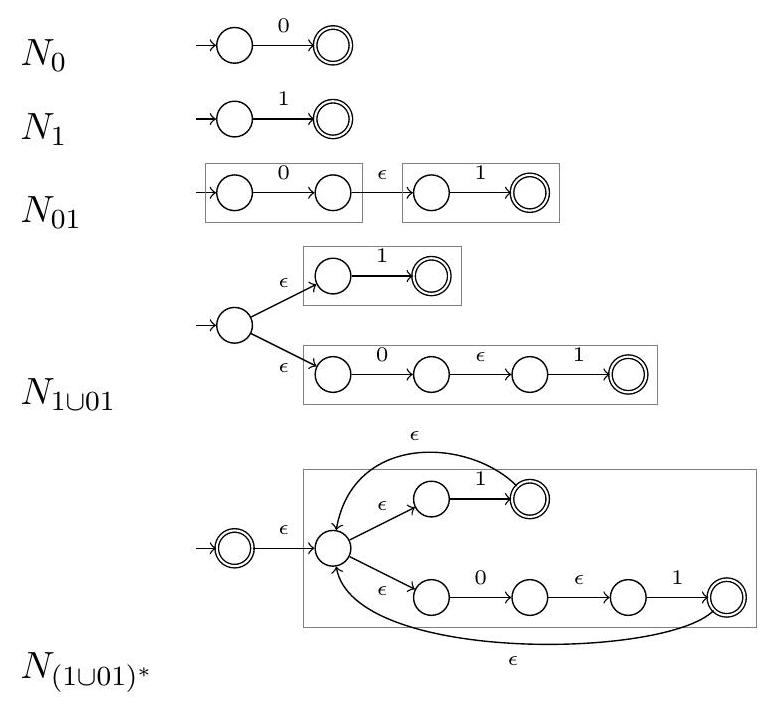
\includegraphics[]{images/regex-to-nfa.jpg}
  }
\end{center}
% \end{multicols*}
\begin{multicols*}{3}
  \section{Definitions}
\subsection{Machine Domains}
\begin{tabular}{|c|c|c|}
  \hline
  DFA \& NFA & PDA & Turing Machines \\
  \hline
  Regex & CFG & Code \\
  \hline
\end{tabular}
\subsection{Finite Automaton}
$M = \left(Q, \Sigma, \delta, q_0, F\right)$

\hspace{5mm}$Q$ set of states

\hspace{5mm}$\Sigma$ alphabet

\hspace{5mm}$\sigma$ transition function

\hspace{5mm}$q_0$ initial state, and $F$ set of final states.

\hspace{5mm}For DFA $\delta: Q\times\Sigma \to Q$

\hspace{5mm}For NFA $\delta: Q\times(\Sigma \cup \{\epsilon\}) \to \mathcal{P}(Q)$
\subsection{Context-Free Grammar}
$G = (V, \Sigma, R, S)$

\hspace{5mm}$V$: variables/non-terminals

\hspace{5mm}$\Sigma$: symbols/terminals

\hspace{5mm}$R$: rules $(A \to \alpha), A\in V, \alpha\in(V\cup\Sigma)^*$

\hspace{5mm}$S$: initial variable, $S\in V$
\subsection{Pushdown Automata}
$M = (Q, \Sigma, q_0, \delta, F, \Gamma)$, NFA + stack

\hspace{5mm}$Q$: states

\hspace{5mm}$\Sigma$: alphabet

\hspace{5mm}$q_0$: starting state

\hspace{5mm}$\delta: Q\times\Sigma\times\Gamma \to \mathcal{P}(Q\times\Gamma)$

\hspace{5mm}\hspace{9mm}pop\rotatebox[origin=c]{270}{$\Lsh$}\hspace{6.8mm}push\rotatebox[origin=c]{270}{$\Lsh$}

\hspace{5mm}$F$: accepting states

\hspace{5mm}$\Gamma$: stack alphabet
\subsection{Turing Machine}
$M = (Q, \Sigma, \Gamma, q_0, q_\mathrm{acc}, q_\mathrm{rej}, \delta)$, DFA + tape

\hspace{5mm}$Q$: control states

\hspace{5mm}$\Sigma$: input alphabet

\hspace{5mm}$\Gamma$: tape alphabet ($\Sigma\subseteq\Gamma$)

\hspace{5mm}$q_0$: initial state

\hspace{5mm}$q_\mathrm{acc}$: accepting state

\hspace{5mm}$q_\mathrm{rej}$: rejecting state

\hspace{5mm}$\delta: Q\times\Gamma\to Q\times\Gamma\times\left\{L, R\right\}$

\hspace{5mm}\hspace{2.6mm}read\rotatebox[origin=c]{270}{$\Lsh$}\hspace{11.5mm}\rotatebox[origin=c]{90}{$\Rsh$}write

A TM first reads input, writes to tape, and moves left or right in that
order. The possible results of a TM is to accept, to reject, or to loop.
Accepting and rejecting means halting.

A machine $M$ that \textbf{recognizes} $L$

\hspace{5mm}$\forall w \in L, M \textrm{ accepts } w$

\hspace{5mm}$\forall w \notin L, M \textrm{ rejects } w \textrm{ or loops}$

A machine $M$ that \textbf{decides} $L$

\hspace{5mm}$\forall w \in L, M \textrm{ accepts } w$

\hspace{5mm}$\forall w \notin L, M \textrm{ rejects } w$

\hspace{5mm}$M$ never loops
\subsection{CFL Closures}
\textbf{Closed}: union, concat, Kleene star, homomorphism, $L\cap R$

\textbf{Not closed}: $L_1\cap L_2$, complement
\subsection{Recursive Enumeration}
An enumerator is a multi-tape TM with output write-only tape. Defined as

$E(M) = \left\{w ~|~ M \textrm{ enumerates } w\right\}$

If for a language $L ~~\exists M$ s.t. $L = E(M)$, then $L$ is recursively
enumerable.

\subsection{Halting Problem}
$\mathrm{HALT} = \left\{\langle M, w \rangle ~|~ M \textrm{ halts on } w\right\}$
is undecidable

\subsection{Language Domains}
Recursive enumeration implies lang is recognizable and vice versa.
Undecidable is the same as not-computable.

\hspace{5mm}Regular

\hspace{10mm}Context-free ($0^n1^n$)

\hspace{15mm}Decidable ($0^n1^n0^n$)

\hspace{20mm}Recursively Enumerable

\hspace{25mm}Undecidable

For reductions $A \leq_m B$ means $A$ is lower or equal in the hierarchy
than $B$. Implications can be drawn depending on what is given.

\subsection{Decidable Closures}
\textbf{Closed}: union, intersection, complement, concat, Kleene star,
and inverse homomorphism.

\textbf{Not closed}: homomorphism
\subsection{Recursively Enumerable Closures}
\textbf{Closed}: union, intersection, concat, Kleene star, homomorphism,
and inverse homomorphism.

\textbf{Not closed}: complement

\subsection{Reductions}
A function $f: \Sigma^\ast \to \Sigma^\ast$ is computable if $\exists$ a
TM that, when given $w$ as input, halts with $f(w)$ on the tape. A
computable reduction is defined as:

$\forall w \in \Sigma^\ast, w\in A \iff f(w)\in B$
  \section{Examples}
\subsection{Regularity of Intersection}
Let $A$ and $B$ be regular languages with alphabet $\Sigma$. Prove that
$A\cap B$ is also regular.

$M_A = (Q_A, \Sigma, \delta_A, q_0^A, F_A)$ \\
$M_B = (Q_B, \Sigma, \delta_B, q_0^B, F_B)$

There exists state machine $M_C$ such that it accepts strings in $A$ and
$B$. It is defined as

$M_C = (Q_A\times Q_B, \Sigma, \delta_C, (q_0^A, q_0^B), F_C)$

where

$\delta_C((q_A, q_B), x) = (\delta_A(q_A, x), \delta_B(q_B, x))$ \\
$F_C = \left\{(q_A, q_B) ~|~ q_A \in F_A \text{ and } q_B \in F_B\right\}$

\subsection{Regularity of Union}
Same as above but the final states use an ``or''

$F_C = \left\{(q_A, q_B) ~|~ q_A \in F_A \text{ or } q_B \in F_B\right\}$

\subsection{Pumping Lemma Setup}
Suppose $L$ is a regular language. Then $\exists p \geq 1$ s.t. $\forall
w \in L$, we can write $w = xyz$, where $|y| \geq 1$, $|xy| \leq p$, and
$xy^iz \in L$ for any $i\in \mathbb{Z}: i \geq 0$.

Let $L = \{0^n 1^m | n < m\}$ for example. We can then define $w$ in
some way that satisfies $L$: $w = 0^p1^{p+1}$. Note that $|w| \geq p$
and $xy=0^p$, so $|xy| \leq p$

Thus we can write $w = xyz$ where

$y=0^j, \quad 1 \leq j \leq p$\\
$x=0^k, \quad 1 \leq k \leq p - j$\\
$z=0^{(p - j - k)}1^{p+1}$

thus $w = 0^k0^j0^{(p-j-k)}1^{p+1}=0^{(k+j+p-j-k)}1^{p+1}=0^p1^{p+1}$

Then we can pump up and let $i=2$

$w^\prime = 0^k0^{2j}0^{(p-j-k)}1^{p+1}=0^{(k+2j+p-j-k)}1^{p+1}=0^{p+j}1^{p+1}$

Because we defined $j$ in such a way that it must be 1 or larger then
$p+j \geq p+1$; therefore $L$ is not regular.

\subsection{Perfect Shuffle (zip)}
For languages $A$ and $B$ over $\Sigma$, let the perfect shuffle be the
language

$\{w | w = a_1b_1 a_2b_2 \dots a_kb_k, 
\text{ where } a_1\dots a_k \in A \text{ and } b_1\dots b_k \in B\}$

Example: suppose that ``rose'' is in language $A$ and ``text'' is in
language $B$, then the string "rtoesxet" is in the perfect shuffle of
$A$ and $B$. Programmers know this more commonly as zipping. Show that
the class of regular languages is closed under perfect shuffle.

Solution: To show that regular languages are closed under perfect
shuffle, it is sufficient to construct an FA that accepts the language
of a perfect shuffle for any regular language $A$ and $B$.

Because $A$ and $B$ are regular, we can construct DFA that accept both
languages. We have DFA $M_1$ for $A$ that has state space $Q_1$ and DFA
$M_2$ for $B$ with state space $Q_2$. The new new DFA for the shuffle
$M_3$ would have state space $Q1\times Q_2\times {0,1}$. The extra set
is to indicate whether to simulate $M_1$ or $M_2$. A state with 0 as the
last member of triple would mean to simulate $M_1$ and a 1 to simulate
$M_2$. The new start state of $M_3$ will be (start of Q1, start of
$Q_2$, 0) to indicate to start by simulating $M_1$. After that $M_3$
will transition to the next state to start simulating $M_2$:

$\delta_{M_3}(~ ( q_{(0,1)}, q_{(0,2)} ), 1^\text{st} \text{ sym}~) = $\\
$(\delta_{M_1}(q_{(0,1)}, 1^\text{st} \text{ sym}), q_{(0,2)}, 1)$

Then $M_3$ will transition to the next state to start simulating $M_1$ again:

$\delta_{M_3}(~ (\delta_{M_1}(q_{(0,1)}, 1^\text{st} \text{ sym}), q_{(0,2)}, 1), 2^\text{nd} \text{ sym} ~) = $\\
$(\delta_{M_1}(q_{(0,1)}, 1^\text{st} \text{ sym}), \delta_{M_2}(q_{(0,2)}, 2^\text{nd} \text{ sym}), 0)$

Thus $M_3$ will go back and forth, simulating the states in $M_1$ and $M_2$. The final states will be (Final States of $M_1$)$\times$(Final States of $M_2$)$\times$0, representing when each part of the string has been accepted by both $M_1$ and $M_2$ after the same number of number of simulations of both $M_1$ and $M_2$.
  % add props of langs and props of TMs
  % add examples of "show decidable"
  % add examples of "show recognizable"
  % add examples of "show undecidable"
  % add examples of "is decidable or undecidable"
\end{multicols*}

% \newpage
% \begin{multicols*}{3}
% \end{multicols*}
\end{document}